%!TEX root = ../thesis.tex

\section{本章の概要}
本章では,\ref{sec:nav-sys}節でシステムの概要を示す.

% \newpage

\section{システム概要}\label{sec:nav-sys}
\figref{Fig:nav-system}に,ナビゲーションシステムの概要図を示す.主に構成しているモジュールを以下に示す.

\begin{itemize}
  \item \textbf{制御モジュール} \\
  制御モジュールは,Navigation Stackの主要コンポーネントであるmove\_baseで構成されている.
  センサデータと目標位置を受け取り,適切なロボットの制御指令を出力する.
  \item \textbf{認識モジュール} \\
  認識モジュールは,YOLOを用いて歩行者の検出及び,追跡を行う.そして,観測時間分のデータをまとめて時系列データとして,独自メッセージで出力する.
  \item \textbf{予測モジュール} \\
  予測モジュールは,認識モジュールからメッセージを受け取り,そのデータを基に\chapref{chap:proposed_method}で述べたネットワークを用いて歩行者の位置予測を行う.その後,制御モジュールのglobal\_costmapの独自レイヤで予測結果をコストマップに反映する.
\end{itemize}

\begin{figure}[hbtp]
  \centering
 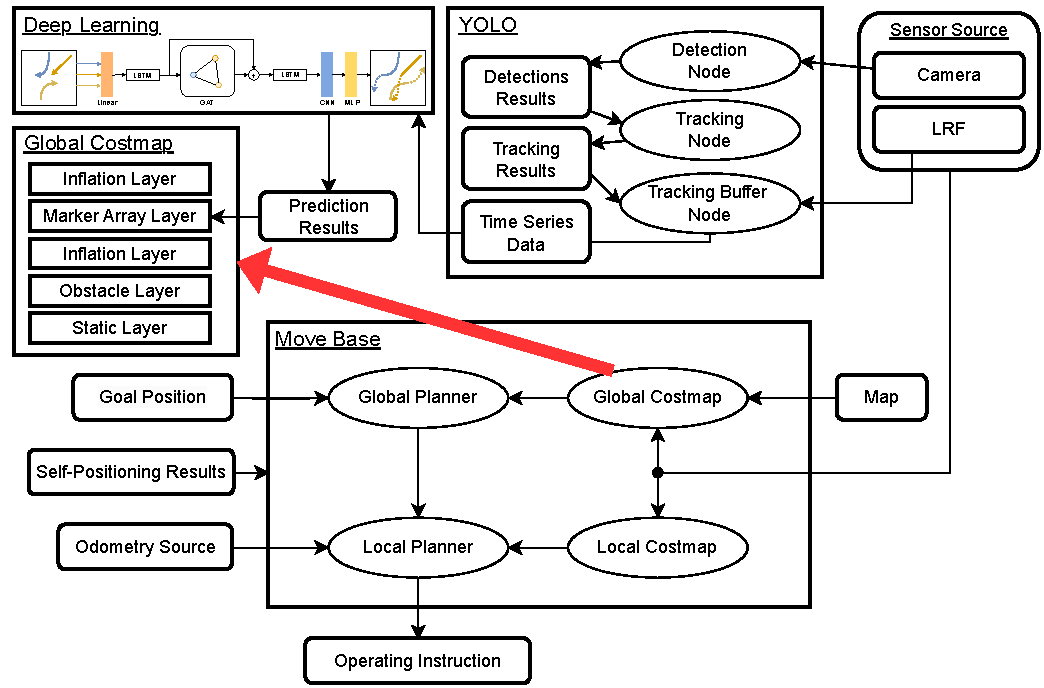
\includegraphics[keepaspectratio, scale=0.77]
      {images/application_system.pdf}
 \caption{Navigation System Overview}
 \label{Fig:nav-system}
\end{figure}  

\section{歩行者の位置推定}

\section{ナビゲーションで予測結果を扱う方法}

\newpage
